\documentclass[8pt]{extarticle}
\title{}
\author{Avinash Iyer}
\date{}

%font setup
%
%\usepackage[math]{anttor}

%paper setup
\usepackage{geometry}
\geometry{letterpaper, portrait, margin=1in}
\usepackage{fancyhdr}

%symbols
\usepackage{amsmath}
\usepackage{amssymb}
\usepackage{hyperref}
\usepackage{gensymb}

\usepackage[T1]{fontenc}
\usepackage[utf8]{inputenc}

%chemistry stuff
\usepackage[version=4]{mhchem}
\usepackage{chemfig}
\usepackage{pdfpages}
%plotting
\usepackage{pgfplots}
\usepackage{tikz}

%\usepackage{natbib}

%graphics stuff
\usepackage{graphicx}
\graphicspath{ {./images/} }

%a useful command
\newcommand{\plain}[1]{\textrm{#1}}

%code stuff
%when using minted, make sure to add the -shell-escape flag
%you can use lstlisting if you don't want to use minted
%\usepackage{minted}
%\usemintedstyle{pastie}
%\newminted[javacode]{java}{frame=lines,framesep=2mm,linenos=true,fontsize=\footnotesize,tabsize=3,autogobble,}
%\newminted[cppcode]{cpp}{frame=lines,framesep=2mm,linenos=true,fontsize=\footnotesize,tabsize=3,autogobble,}

\usepackage{listings}
\usepackage{color}
\definecolor{dkgreen}{rgb}{0,0.6,0}
\definecolor{gray}{rgb}{0.5,0.5,0.5}
\definecolor{mauve}{rgb}{0.58,0,0.82}

\lstset{frame=tb,
	language=Java,
	aboveskip=3mm,
	belowskip=3mm,
	showstringspaces=false,
	columns=flexible,
	basicstyle={\small\ttfamily},
	numbers=none,
	numberstyle=\tiny\color{gray},
	keywordstyle=\color{blue},
	commentstyle=\color{dkgreen},
	stringstyle=\color{mauve},
	breaklines=true,
	breakatwhitespace=true,
	tabsize=3
}
% text + color boxes
\usepackage{tcolorbox}
\newtcolorbox{mathbox}[1]{title = {#1}}

\pagestyle{fancy}
\fancyhf{}
\rhead{Ling Chen, Avinash Iyer, Nora Manukyan, Vincent Ng}
\lhead{Homework Section 1.1: Group A Problems}
\begin{document}
\begin{mathbox}{Problem 1.1.13}
    Let $G$ be the graph whose vertex set is the set of $k$-tuples with coordinates $\{0,1\}$, with $x$ adjacent to $y$ if $x$ and $y$ differ by exactly one position. Determine whether $G$ is bipartite.
  \end{mathbox}
  \noindent $G$ is bipartite --- we can find a bipartition by separating the set into a set of tuples which differ by an even number of positions and a set of tuples which differ by an odd number of positions. Since odd numbers differ from each other by at least $2$ places, and even numbers differ from each other by at least $2$ places, we know that each subset of tuples is not adjacent to each other, but is adjacent to the other set. 
\begin{mathbox}{Problem 1.1.26}
     Let $G$ be a graph with girth $4$ in which every vertex has degree $k$. Prove that $G$ has at least $2k$ vertices. Determine all such graphs with $2k$ vertices. 
  \end{mathbox}
  \noindent Suppose $G$ is a graph with girth $4$ with every vertex of degree $k$. Let $v_i\in V(G)$. Then, there must be $k$ vertices which $v_i$ is adjacent to. However, none of these vertices can be adjacent to themselves or $G$ would have girth $3$. Thus, we can form a bipartition such that $v_i$ is in a set of at least $k$ vertices such that each vertex is not adjacent to itself, and each vertex in this set is adjacent to $k$ vertices in a disjoint set where each vertex in this set is not adjacent to any other vertex in this set. Therefore, there are at least $2k$ vertices.\\

  \noindent The graphs with exactly $2k$ vertices are the $K_{n,n}$ complete bipartite graphs.

\begin{mathbox}{Problem 1.1.27}
    Let $G$ be a graph with girth 5. Prove that if every vertex of $G$ has degree at least $k$, then $G$ has at least $k^2+1$ vertices. For $k=2$ and $k=3$, find one such graph with $k^2+1$ vertices.      
  \end{mathbox}
  \noindent Let $G$ be a simple graph with girth 5. Suppose that every vertex of $G$ has degree $k$. Let $u\in V(G)$. Then, $u$ has $k$ adjacent vertices, each of which is not adjacent to each other (or else the girth of $G$ would be $3$). Let this set be $N$. The elements of $N$ cannot have any other common neighbors aside from $u$, or else the girth of $G$ would be $4$, meaning each has $k-1$ distinct neighbors. Therefore, the total number of vertices in our graph includes $u$, the elements of $N$ that are the $k$ distinct neighbors of $u$, and the $k(k-1)$ distinct vertices for each vertex in $N$. Therefore, our total is $1 + k + k(k-1) = k^2 + 1$.\\

  \noindent If there were any vertex with degree greater than $k$, then there would be additional vertices beyond the $k^2 + 1$ vertices necessary for a $k$-regular graph.\\

  \noindent For  $k=2$, we have the graph $C_5$ for an example of a graph with $k^2 + 1$ vertices, and for $k=3$ we have the Petersen graph.
\begin{mathbox}{Problem 1.1.30}
    Let $G$ be a simple graph with adjacency matrix $A$ and incidence matrix $M$. Prove that the degree of $v_i$ is the $i$th diagonal entry of $A^2$ and $MM^T$. What do the entries in position $(i,j)$ of $A^2$ and $MM^T$ say about $G$?
  \end{mathbox}
  \noindent Let $A$ be the adjacency matrix for a simple graph $G$. In $A$, every vertex's corresponding row and column are identical, meaning that the entry $A^2_{i,i}$ will be equal to $r_ic_i$ for row $i$ and column $i$ corresponding to $v_i$. Thus, $r_ic_i$ is equal to $|c_i|^2$, which is equal to the sum of the elements of $c_i$, which is equal to the degree of $v_i$.\\

  \noindent Let $M$ be the incidence matrix for a simple graph $G$. In $MM^T$, the diagonal element $MM^T_{i,i}$ will be equal to $r_i r_i^T$, where $r_i$ represents the edge incidence row of $v_i$. This is equal to $\left|r_i^T\right|^2$, which is equal to the sum of the elements of $r_i$, which is equal to the number of edges incident on $v_i$, which is equal to the degree of $v_i$.\\

  \noindent The entry in position $(i,j)$ in both $A^2$ and $MM^T$ shows whether vertices $v_i$ and $v_j$ are adjacent to each other.
\begin{mathbox}{Problem 1.1.34}
    Decompose the Petersen graph into three connected subgraphs that are pairwise isomorphic. Also decompose it into copies of $P_4$.
  \end{mathbox}
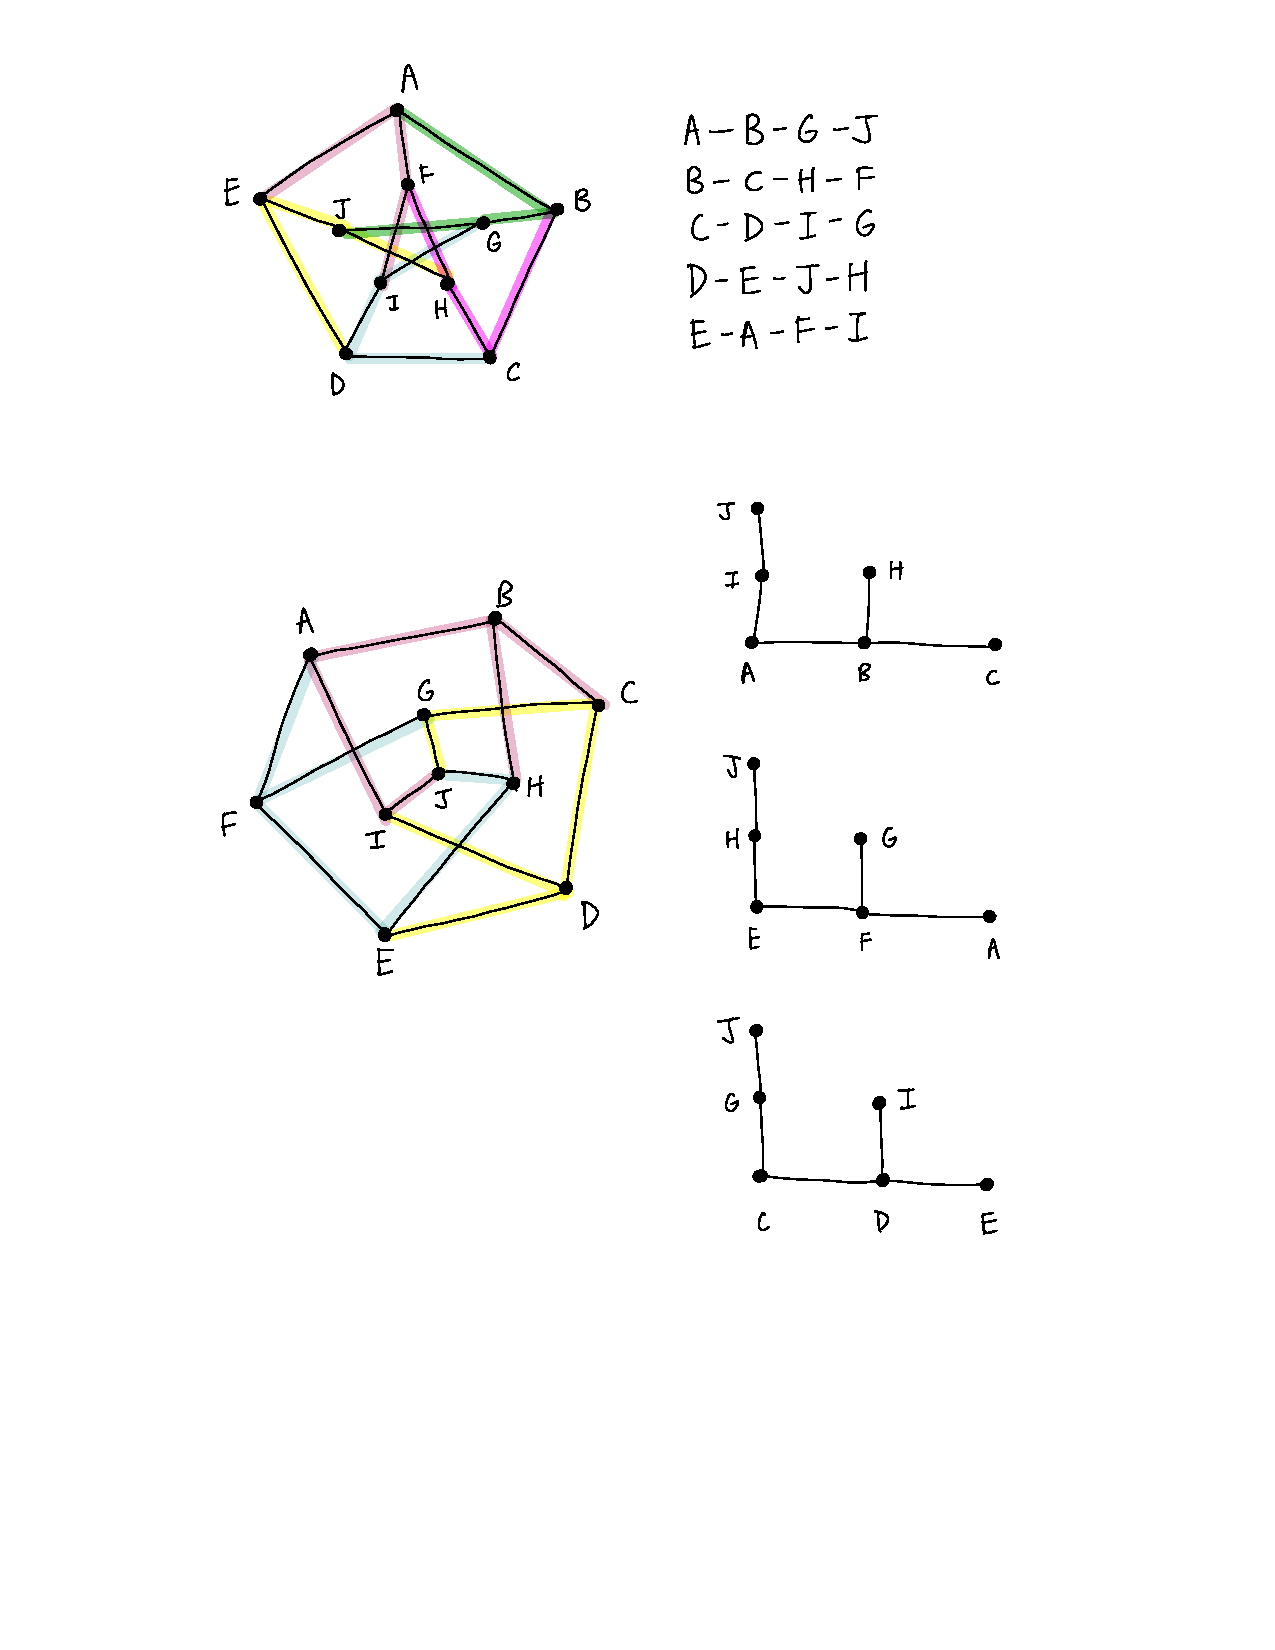
\includepdf{images/1_1_34.pdf}
\end{document}
